\documentclass[]{article}


\usepackage[utf8]{inputenc}
\usepackage{listings}
\usepackage{hyperref}
\usepackage{float}
\usepackage{graphicx}
\usepackage{subfig}
\graphicspath{ {imagenes/} }
\usepackage{xcolor}
\definecolor{RoyalBlue}{cmyk}{1, 0.50, 0, 0}
\usepackage{listings}
\lstset{language=Java,
keywordstyle=\color{RoyalBlue},
basicstyle=\scriptsize\ttfamily,
commentstyle=\ttfamily\itshape\color{gray},
stringstyle=\ttfamily,
showstringspaces=false,
breaklines=true,
frameround=ffff,
frame=single,
rulecolor=\color{black}}



%opening
\title{Practica 3 TSI}
\author{José Manuel Pérez Lendinez}

\begin{document}

\maketitle


\newpage
\tableofcontents
\newpage
\section{Ejercicio 1}
El siguiente problema a resolver (problema-zeno-V01.pddl) consiste en transportar 3 personas (inicialmente en las ciudades C1, C2 y C3) a la ciudad C5, considerando que el avión está en la ciudad C4.
Se asume al igual que en el problema ejemplo que no hay restricciones de fuel.

El problema en este ejercicio viene dado porque no teníamos en cuenta que el avión y el pasajero no estén en la misma ciudad. Esto lo solucionamos añadiendo un nuevo método que llamara a un avión que esta situado en otra ciudad. 

Cuando se cumpla este caso se llamara a el avión a la ciudad donde se encuentra el pasajero, se hará el board y se mandara el avión a la cidudad destino
\begin{figure}[H]
	\centering
	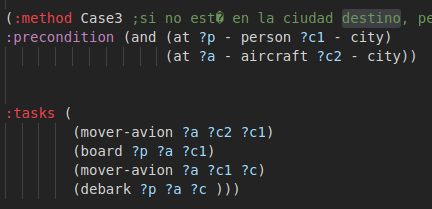
\includegraphics[width=0.7\linewidth]{screenshot002}
	\caption{}
	\label{fig:screenshot002}
\end{figure}

\section{Ejercicio 2}
En este caso tendremos que añadir las opciones necesarias para tener en cuenta el fuel de un avión. En este caso se tendrá que tener en cuenta que para ir de una ciudad a otra necesitaremos tener le fuel necesarios. Para esto crearemos un derived que nos devuelva el verdadero cuando tengamos fuel suficiente para ir de una ciudad a otra.
\begin{figure}[H]
	\centering
	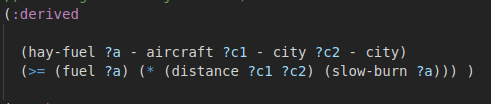
\includegraphics[width=0.7\linewidth]{screenshot003}
	\caption{}
	\label{fig:screenshot003}
\end{figure}

Con esto ya podemos modificar el task mover avión utilizando esta función. Se tendrá dos method uno cuando tengamos fuel que simplemente realizara el fly y otro en el caso de no tener fuel donde se realizara un refuel antes del fly.
\begin{figure}[H]
	\centering
	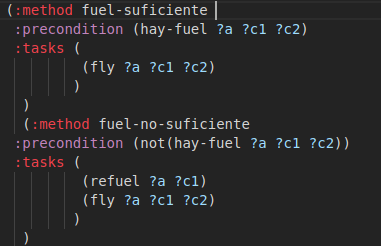
\includegraphics[width=0.7\linewidth]{screenshot004}
	\caption{}
	\label{fig:screenshot004}
\end{figure}

\section{Ejercicio 3}
En este caso se tendrá que diferenciar entre le vuelo rápido y lento. Dándole prioridad a los vuelos rápidos. Se tiene que añadir un nuevo derived igual que en el ejercicio anterior, con la diferencia de que tendrá en cuenta cuanto gasta un vuelo rápido en vez de uno lento.
\begin{figure}[H]
	\centering
	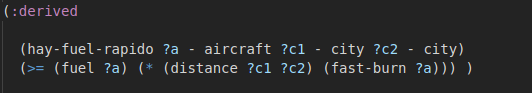
\includegraphics[width=0.7\linewidth]{screenshot006}
	\caption{}
	\label{fig:screenshot006}
\end{figure}
El derived del ejercicio anterior le cambiaremos el nombre ha hay-fuel-rápido.

También tendremos que tener dos nuevos derived para comprobar si sobrepasamos el limite máximo de fuel que se definirá para este ejercicio. Uno de ellos comprobara si lo sobrepasamos volando rápido y el otro volando lento.
\begin{figure}[H]
	\centering
	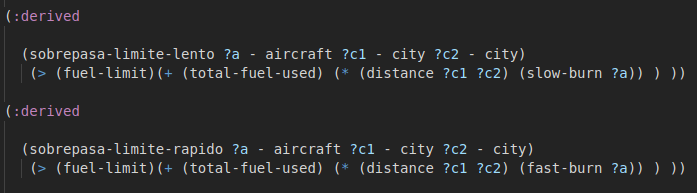
\includegraphics[width=0.7\linewidth]{screenshot007}
	\caption{}
	\label{fig:screenshot007}
\end{figure}

Una vez tengamos las funciones preparadas podremos modificar en método mover-avion para darle prioridad a los vuelos radios. Para esto podremos primero los task que realizan el vuelo rápido y los últimos los task que realizan los vuelos lentos. Primero iran los method de vuelo rapido. Donde se usara las funciones que tendra en cuenta que no sobrepasa el limite y que tenemos fuel al volar rapido.
\begin{figure}[H]
	\centering
	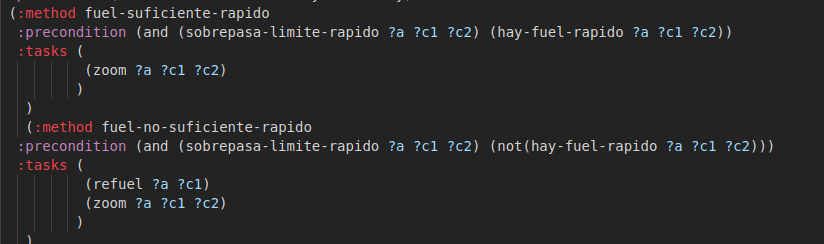
\includegraphics[width=0.7\linewidth]{screenshot008}
	\caption{}
	\label{fig:screenshot008}
\end{figure}

Después de estos dos se tendrán los dos de vuelo lento para ello las funciones de vuelo lento.
\section{Ejercicio 4}
En este caso tendremos un limite de pasajeros por avión que lo representaremos con un predicado (= (limite-pasajeros a1) 10) y otro para representar el numero de pasajeros ya montados que sera (= (personas-montadas a1) 0). A1 representaría  a ana avión. 
Se cambiara las primitivas board y debark para tener en cuenta el limite de pasajeros. En board añadiremos una nueva restricción para que sola pueda aumentar pasajeros cuando no se supere limite y incremente el predicado personas-montadas. En el caso de debark se tendría que diminuir el predicado, no miraremos si estamos por debajo de 0 porque para llamar a un debark el pasajero tendrá que estar en el avión y por tanto anteriormente se ha dado un board.
\begin{figure}[H]
	\centering
	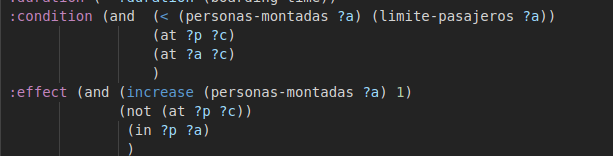
\includegraphics[width=0.7\linewidth]{screenshot009}
	\caption{Board}
	\label{fig:screenshot009}
\end{figure}

\begin{figure}[H]
	\centering
	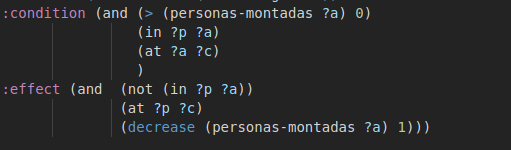
\includegraphics[width=0.7\linewidth]{screenshot010}
	\caption{Debark}
	\label{fig:screenshot010}
\end{figure}

Para poder embarcar varios pasajeros en una misma avión vamos a realizar una función recursiva que sera la encargada de realizar todo lo relacionado con embarcar, desembarcar y movimiento de aviones. Esta función tendrá un total de 5 method. Seran los siguientes: 
\begin{enumerate}
	\item Montado en avión y avión en ciudad destino: En este caso el avión ya se encuentra en la ciudad de destino y el pasajero esta montado en le avios. Se realizara un debark en esta ciudad.
	\begin{figure}[H]
		\centering
		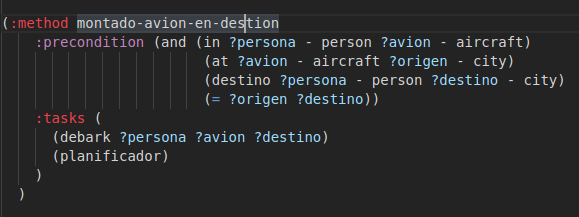
\includegraphics[width=0.7\linewidth]{screenshot011}
		\caption{}
		\label{fig:screenshot011}
	\end{figure}
	
	\item No montado en avión y avión en la ciudad: En este caso sera en el que los pasajeros hagan el board para subir a el avión. Se mirara que la ciudad no sea destino y que el pasajero y el avión estén en la misma ciudad.	
	\begin{figure}[H]
		\centering
		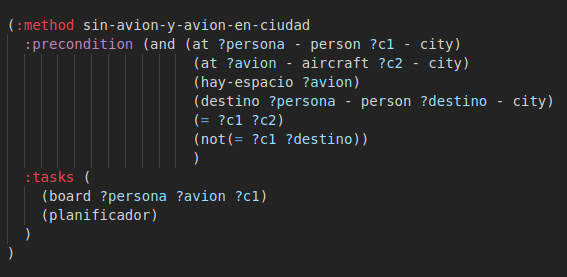
\includegraphics[width=0.7\linewidth]{screenshot012}
		\caption{}
		\label{fig:screenshot012}
	\end{figure}
	
	\item No montado en avión y sin avión en esa ciudad: En este caso se llamara a un avión para que llegue a la ciudad en la que esta el pasajero sin montar en ninguna avión y cuando esa ciudad no sea su destino.
	\begin{figure}[H]
		\centering
		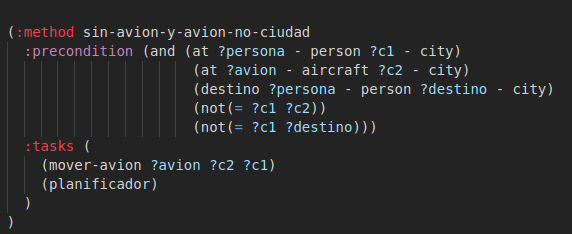
\includegraphics[width=0.7\linewidth]{screenshot015}
		\caption{}
		\label{fig:screenshot015}
	\end{figure}
	
	\item Montado en avión y avión no esta en destino: En este caso el pasajero estará montado en un avión y esta avión estará en una ciudad que no concuerda con la ciudad destino del pasajero. Se realizara un vuelo hasta la ciudad de destino del pasajero.
	\begin{figure}[H]
		\centering
		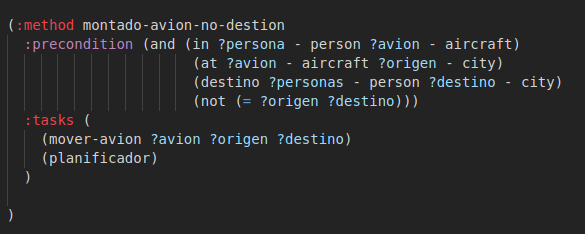
\includegraphics[width=0.7\linewidth]{screenshot014}
		\caption{}
		\label{fig:screenshot014}
	\end{figure}
	
	\item En Destino: Es el caso base en el que no se volverá a realizar la recursividad. Se da cuando el pasajero esta en destino y no esta subido en un avión.
	\begin{figure}[H]
		\centering
		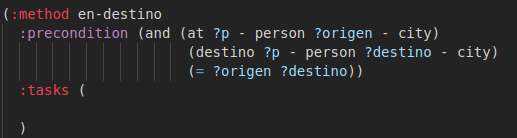
\includegraphics[width=0.7\linewidth]{screenshot013}
		\caption{}
		\label{fig:screenshot013}
	\end{figure}
	
\end{enumerate}

No he realizado la parte de que cada avion tenga un tiempo limite.







	










\end{document}
